\pdfoutput=1
% =====================================================================
% Architecture and design rationale of the MathFin autoformalization
% pipeline. Paper-style technical manual for a formal-methods + ML
% audience. Compiles with: latexmk -pdf autoformalization-pipeline.tex
% (or pdflatex twice). Figure 1 is leanstral-architecture.png in this dir.
% =====================================================================
\documentclass[11pt]{article}

\usepackage[utf8]{inputenc}
\usepackage[T1]{fontenc}
\usepackage[sc]{mathpazo}         % Palatino text + matching math
\renewcommand{\ttdefault}{txtt}   % cleaner monospace for Lean identifiers
\linespread{1.05}
\usepackage[a4paper,margin=1in]{geometry}
\usepackage{amsmath}
\usepackage{amssymb}
\usepackage{booktabs}
\usepackage{array}
\usepackage{graphicx}
\usepackage{microtype}
\usepackage{titlesec}
\titleformat{\section}{\large\scshape}{\thesection}{0.8em}{}
\titleformat{\subsection}{\normalsize\scshape}{\thesubsection}{0.7em}{}
\usepackage[hidelinks]{hyperref}

% Lean identifiers and file names, set in typewriter. \lean allows a line
% break after each underscore so long identifiers wrap; \leanw keeps them whole.
\newcommand{\lean}[1]{\texttt{\def\_{\textunderscore\allowbreak}#1}}
\newcommand{\leanw}[1]{\texttt{#1}}

\title{Architecture of an Autonomous Autoformalization Pipeline\\
  for a Lean~4 Mathematical-Finance Library}
\author{Raphael Coelho\thanks{Independent researcher.
  ORCID: \href{https://orcid.org/0009-0001-6601-1023}{0009-0001-6601-1023}.
  Correspondence: \texttt{raphaelrrcoelho@gmail.com}.
  Library artifact: \url{https://github.com/raphaelrrcoelho/formal-mathfin}.}}
\date{July 2026}

\begin{document}
\maketitle

\begin{abstract}
We built a system that keeps a formally verified library of mathematical finance in
Lean~4 growing without much supervision. It reads the project's own backlog of issues,
drafts a Lean statement for one, proves it, and opens a pull request that has already
passed the kernel; a person only reviews and merges. Two decisions do most of the work.
The first is to use two language models rather than one, split by what each is good at:
a frontier reasoning model drafts each statement---deciding what the theorem should say,
writing it in Lean against a live language server, and breaking a hard one into
lemmas---while a Lean-specialised model proves it. The second is to
check that a drafted statement means what the issue asked \emph{before} putting a prover
on it, because the usual way autoformalization goes wrong is a statement that compiles
but says the wrong thing. What we accept is defined mechanically: the proof elaborates
with no \lean{sorry}, its axioms stay inside the three that Lean and Mathlib already
assume, and a build check holds it there. The paper walks through each stage and the
reason it is built the way it is. This is infrastructure and method, not a result in
finance or in machine learning.
\end{abstract}

\section{Introduction}

Most autoformalization research is built around benchmarks: a fixed set of problems,
each a statement to translate or a lemma to prove, scored in
aggregate~\cite{wu2022autoform,jiang2023draft}. Maintaining a real library is a
different job. The work does not arrive as statements. It arrives as a backlog of things
someone wants to be true, and each has to become a faithful Lean statement, get proved,
and merge into a corpus that other proofs already build on. The failure modes shift with
it. ``Couldn't prove it'' is the mild case. The expensive cases are proving the wrong
statement, proving a true-but-empty restatement, and re-deriving something the library
already contains.

We describe the system we run for \emph{MathFin}, a Lean~4 library of mathematical
finance with more than three hundred \lean{sorry}-free theorems across eleven areas,
built on Mathlib~\cite{mathlib2020} and R\'emy Degenne's \lean{BrownianMotion}
package~\cite{brownianMotion}. It takes GitHub issues in and puts pull requests out, and
between the two it runs on its own.

A few choices shape it, and each gets a section. We split the drafting from the proving
across two models (\S\ref{sec:engines}). We check a statement for faithfulness before
proving it rather than after (\S\ref{sec:gates}). We prove in one long interactive
session instead of many blind attempts, and fall back to decomposition when that is not
enough (\S\ref{sec:prove}). We make acceptance a mechanical bar rather than a human
glance at green output (\S\ref{sec:accept}). And we leave the last word to a person: the
kernel decides what is allowed in, a review decides what is worth keeping
(\S\ref{sec:ship}). Figure~\ref{fig:arch} is the whole pipeline at once;
\S\ref{sec:principles} draws out what recurs and \S\ref{sec:limits} says where it gets
stuck today.

\section{Setting}\label{sec:setting}

Some of the design is forced by the setting rather than chosen.

\subsection{The library is the artifact}
What matters is the library, not the machinery that fills it. So the output has to meet
the library's standards. It should use the Mathlib and \lean{BrownianMotion}
declarations that already exist instead of re-deriving them, and it should read like Lean
a maintainer would have written. That standard, which we call coherence-first, comes
back in the drafter, in the gates, and at review. Everything is pinned to a fixed Lean
toolchain, Mathlib revision, and \lean{BrownianMotion} revision, so that ``it verified''
is a reproducible fact and not a report about one machine on one day.

\subsection{Two repositories}
The engine and the library are separate repositories. The library is public and is where
pull requests land; the engine is a private repository that drives the models, the
gates, and the Lean process. Keeping them apart is deliberate. The library's history
should read as a record of mathematics and its review, not of an orchestration system
being tuned, and we can rework the engine without disturbing the artifact's provenance.
The only thing that crosses between them is a pull request, which has the useful side
effect that the human review cannot be skipped, since there is no other way in.

\subsection{The models are remote; Lean is local and runs one at a time}
The language models are a remote API. The only heavy thing running locally is Lean, and
a Mathlib-loaded Lean process takes several gigabytes, so two of them will not fit on a
modest host. The pipeline holds a strict rule: one Lean-loaded process at a time. A
long-lived Lean server keeps the environment warm between requests, which is the
difference between a check that takes seconds and one that takes minutes, and it is what
makes a tight draft-check-repair loop usable. Runs are token-paced, with one issue per
scheduled tick, a ceiling per issue, and a monthly allowance, so an unattended loop
cannot spend without limit.

\section{Two models}\label{sec:engines}

We use two models. One is a frontier reasoning model, Anthropic's
Claude~\cite{anthropicClaude}; the other, Mistral's Leanstral~\cite{leanstral2026}, is
specialised for Lean. Each takes the part of the work it handles better: the reasoner
drafts, the specialist proves.

The split came from noticing where drafting actually breaks. Ask one model to go straight
from an informal issue to a proved Lean theorem and the failures are almost never in the
mathematics. They are in the Lean: an identifier it guessed at, a coercion it got wrong,
an unbound universe, a binder in the wrong place. The fix is not to hand the Lean to a
different model but to give the drafter the feedback a prover gets: the reasoning model
writes its Lean in an interactive session against the language server, reading each
elaboration error and fixing it, so it produces Lean that elaborates rather than Lean
that merely looks right. Proving---a longer, more search-heavy job---we keep with the
Lean-specialist model trained for it.

The reasoning model does four things: it drafts the \emph{intent} for a statement, it
writes that intent into elaborating Lean (\S\ref{sec:drafter}), it splits a hard target
into lemmas (\S\ref{sec:prove}), and it judges whether a draft is faithful
(\S\ref{sec:gates}). The Lean model does the proving, and runs the two kernel probes that
try to refute a draft (\S\ref{sec:gates}).

\begin{figure}[p]
  \centering
  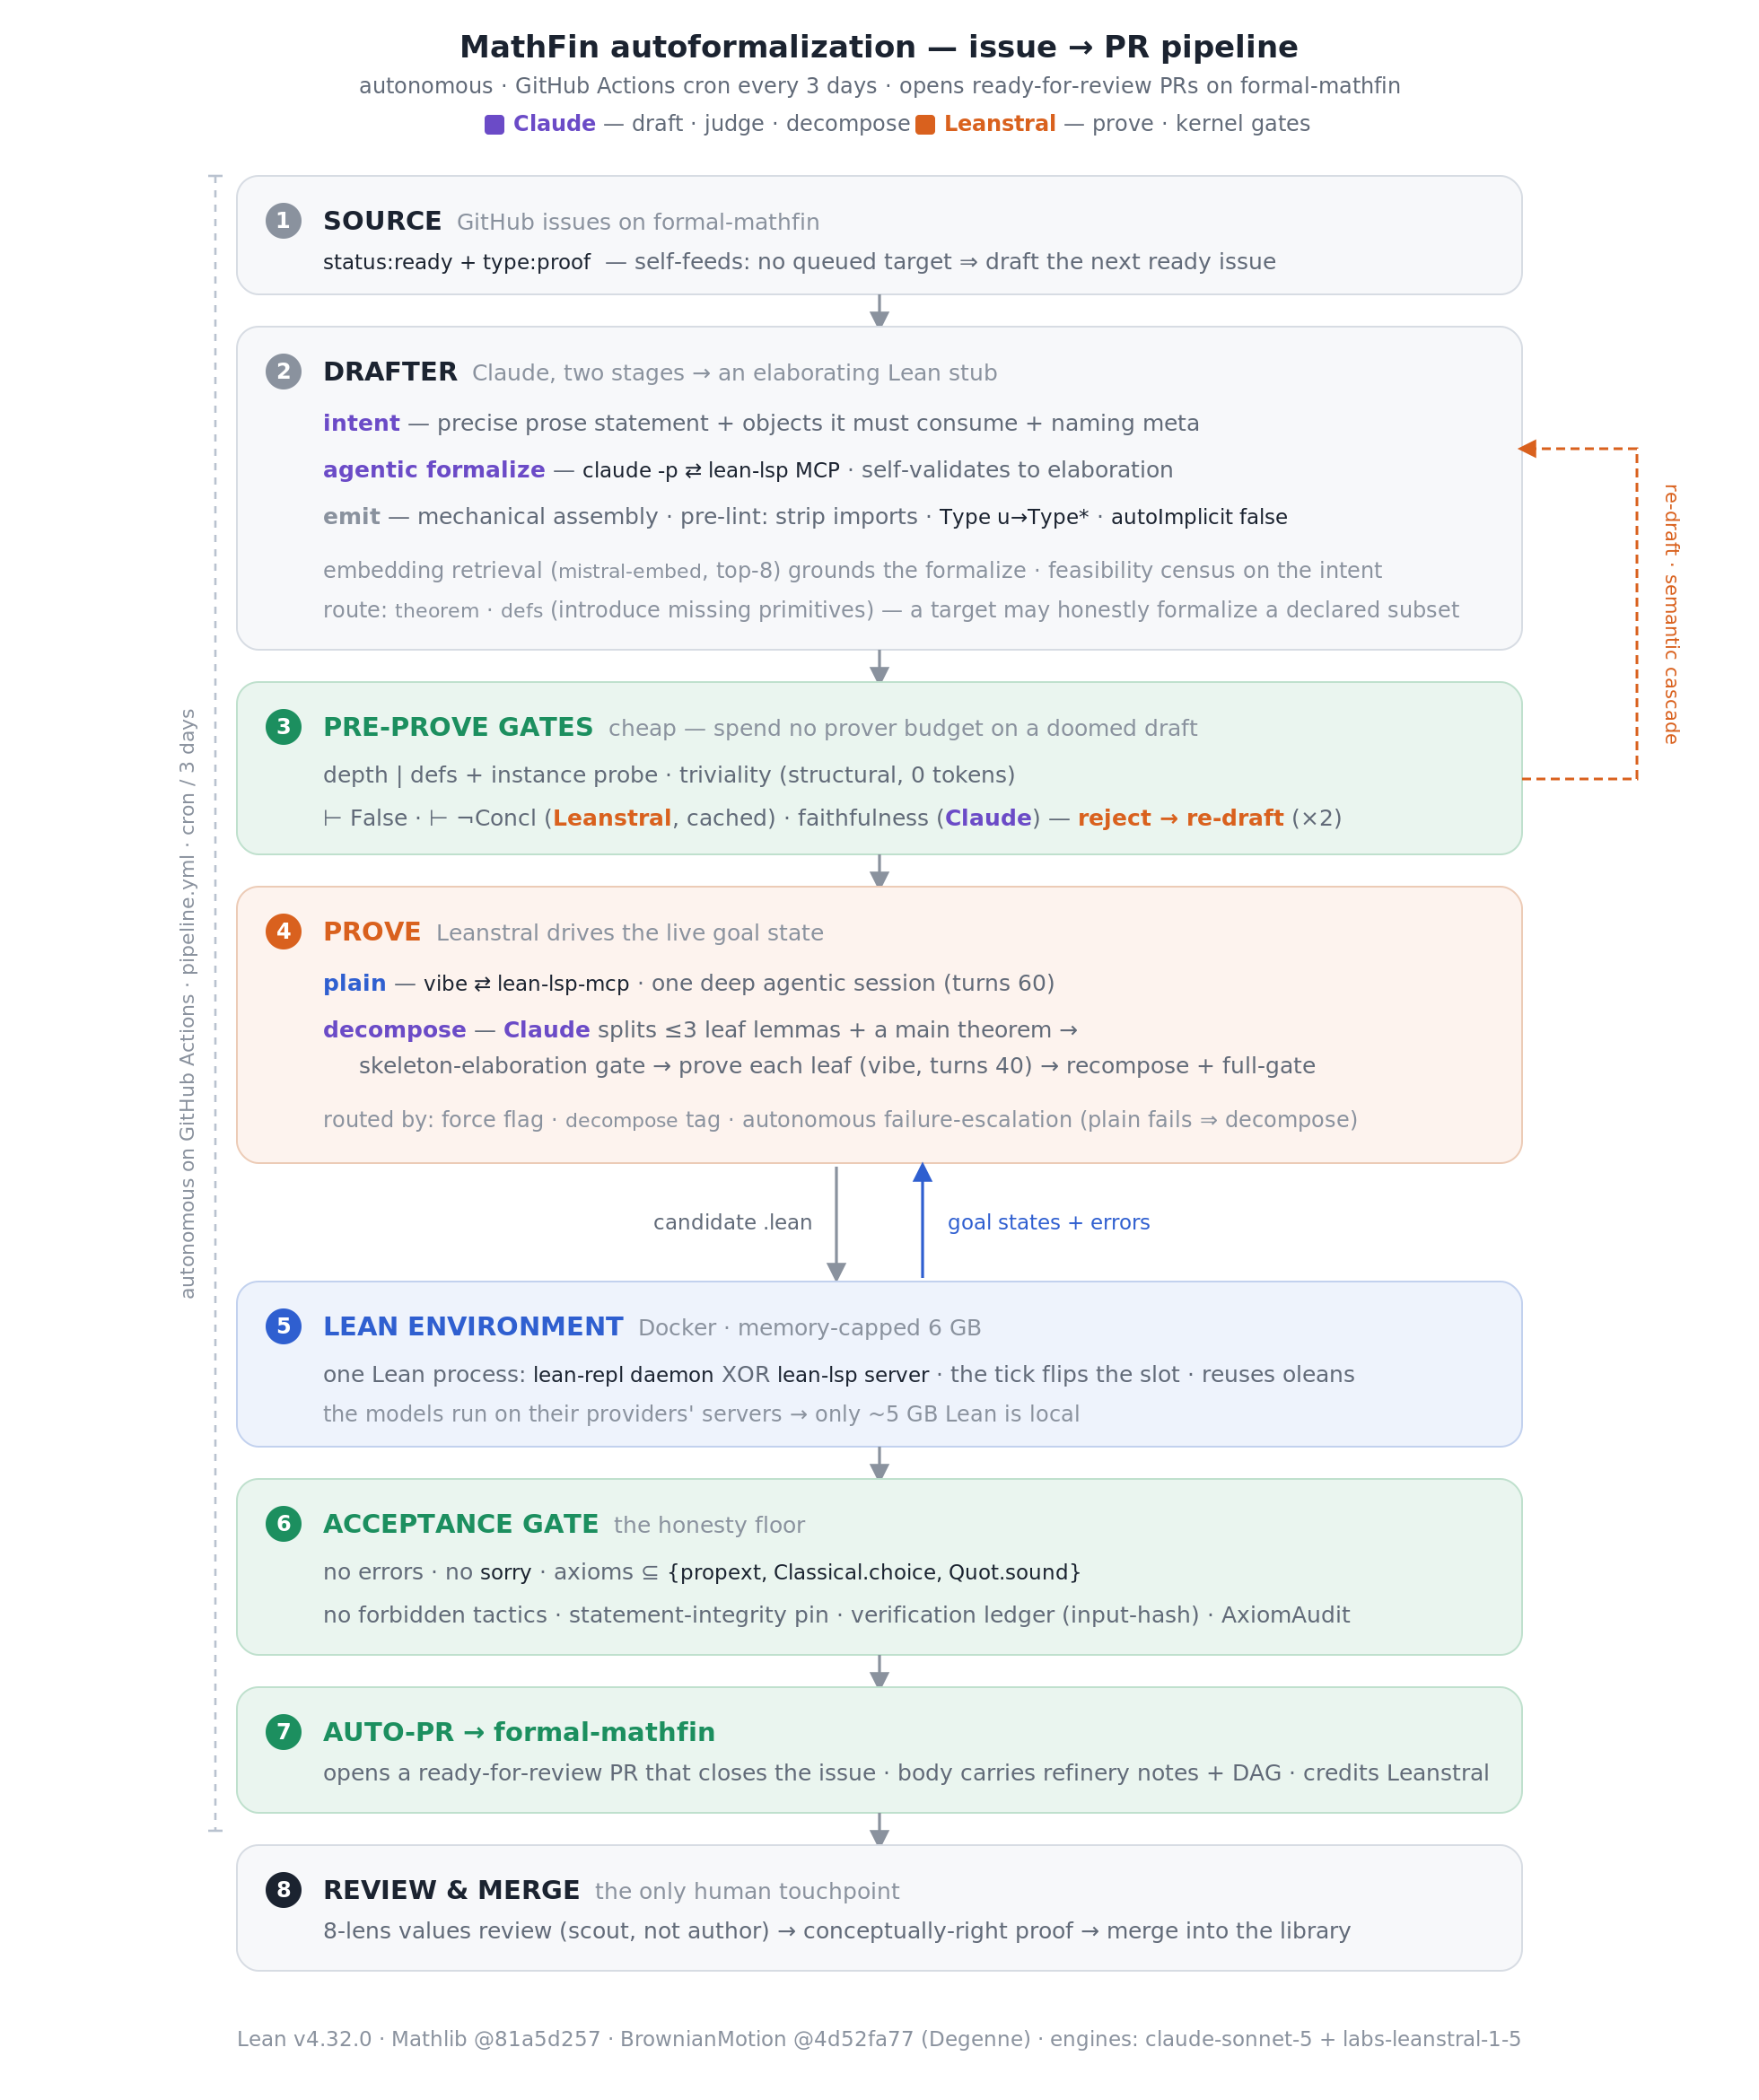
\includegraphics[width=0.9\textwidth]{leanstral-architecture.png}
  \caption{The pipeline end to end. Stages 1--7 run unattended on continuous
  integration; stage~8 is the only human touchpoint. The reasoning model (Claude) and
  the prover (Leanstral) recur across stages in the roles of \S\ref{sec:engines}.
  The dashed return on the right is the repair cascade (\S\ref{sec:gates}); the two-way
  link between \textsc{prove} and the Lean environment is the live goal-state loop
  (\S\ref{sec:prove}).}
  \label{fig:arch}
\end{figure}

\section{Where the work comes from}\label{sec:source}

The unit of work is a GitHub issue, specifically one labelled \emph{ready} and
\emph{proof}. Issues are already where the project writes down what it wants done, in
prose meant for people, and a proof that lands closes its issue the way any contribution
would. That is reason enough to build on them instead of inventing a separate task
format.

The queue feeds itself. Each scheduled tick looks for a target that has already been
drafted; if there is none, it drafts one from the next ready issue and carries on. Nobody
has to stage work ahead of it. An empty queue just means: draft the next issue.

\section{The drafter}\label{sec:drafter}

The drafter turns an issue into a Lean module with a single well-typed theorem statement
ending in \lean{sorry} (an \emph{elaborating stub}). Three things happen inside it.

\subsection{Two stages}
First, \emph{intent}: the reasoning model writes down in prose exactly the theorem to
formalise (every hypothesis, the whole conclusion, the objects it should be built from,
and a little naming metadata), and writes no Lean. Second, \emph{formalise}: the same
model turns that into a single elaborating theorem in an interactive session against the
language server (\S\ref{sec:engines}), playing edits and reading each elaboration error
until the stub is well-typed. Both stages are the reasoning model; the split from the
prover comes after, at \textsc{prove}.

\subsection{Grounding by retrieval}
Formalising well means knowing which declarations to name. We ground the drafter with
premises pulled from the pinned corpus, much as retrieval-augmented provers
do~\cite{yang2023leandojo}: the declarations' type signatures are indexed, queried by
embedding similarity, and the closest matches are handed over as signatures the statement
may use. The point is to draft coherently, to write \lean{MathFin.zcb} instead
of re-inlining a bond price, and, when the model names something that does not exist, to
put the right declaration in front of the repair loop. If the index happens to be
missing, retrieval falls back to name-based search, so a cold cache slows a draft but
never blocks it.

\subsection{A mechanical, deterministic emit}
Assembling the module (licence header, imports, the pinned build options, the namespace,
the statement itself) is mechanical and uses no model call. One thing is worth doing here
rather than in a prompt: fixing the model's systematic tics with a small deterministic
pass. The drafter likes to prepend an \lean{import} line, which is illegal partway
through a module, so we strip it. It sometimes writes an explicit universe variable the
build options forbid, so we rewrite it to the anonymous form. It writes measure-theory
names bare, the way a file that has already opened those namespaces would, so we open
them. The rule behind all three is the same: when a mistake is systematic and you can
describe it mechanically, fix it in code, not by asking the model again and hoping.

\subsection{Routes, and covering only part of an issue}
Not every issue is one theorem over things that already exist. So the drafter has two
routes. The ordinary one states a result through existing declarations; the \emph{defs}
route first introduces the one to three new definitions the statement needs, each built
from constants already in the library. A draft may also cover only part of a multi-part
issue on purpose, as long as it says so. The facts it leaves out are recorded and become
follow-up issues, so a partial result is visible as one rather than passing for the whole.

\section{Checking before proving}\label{sec:gates}

An agentic proving session is the most expensive thing the pipeline does, so a draft that
is infeasible, unfaithful, shallow, or empty should never reach one. A short stack of
checks runs first, each costing at most one elaboration or one quick model call, and only
what survives is handed to the prover.

\emph{Feasibility.} If the intent names library primitives that do not exist, the draft
is rejected and sent to the defs route or to a person; drafting against invented
constants is the quickest way to waste a proving budget. \emph{Faithfulness.} The
reasoning model reads the issue against the Lean and rejects a draft that says the wrong
thing: a hypothesis missing, an inequality flipped, a conjunct quietly dropped.
\emph{Depth.} A statement whose type touches none of the domain primitives it claims to
be about is usually a generic Mathlib identity in disguise, and is rejected.
\emph{Triviality.} A statement that a one-line \lean{rfl} or \lean{simp} closes is a
restatement of a definition with no content, and is rejected.

The reason these matter is that the kernel is no help against them. A wrong statement
that happens to be provable passes the kernel cleanly; the error is in what was asked,
not in the proof. The gates are the only place that kind of error is caught, and they
catch it before a prover has spent anything.

A rejection is not the end of it. The verdict is usually specific (a named missing
hypothesis, or ``this is the Sharpe ratio, not the Omega ratio''), so we hand it back and
let the drafter try again with the criticism in view, for a few rounds. That makes the
stack a loop rather than a wall.

\section{Proving}\label{sec:prove}

\subsection{One deep session}
The prover is the Lean model working an interactive session through a language-server
interface~\cite{leanlspmcp}: it plays a tactic, reads the new goal state, hovers for a
type, checks a diagnostic, searches for a lemma, all live. One target gets one long
session with a turn budget, not a batch of blind samples. The reasoning is
straightforward. A model that sees the goal after each step is in roughly the position a
human prover is in, and for a fixed budget a single session that can react beats many
short ones that cannot. When we want the prover to try harder on a target, the turn
budget is the dial we turn.

\subsection{Decomposition}
Some goals are too big for one session. For those, the reasoning model splits the target
into a few named leaf lemmas (at most three) and a main theorem that uses them, a shallow
DAG. Before any leaf gets a proving budget, a skeleton check confirms the assembled split
elaborates and carries exactly the leaf \lean{sorry}s it should, so a badly shaped split
costs one elaboration to reject instead of several proving sessions to discover. Each leaf
is then proved as an ordinary single-\lean{sorry} target by the same prover, and a final
check reassembles the whole and runs it through the full acceptance bar. Decomposition
gets past the length a single session can handle without changing anything about how the
session works, and the cost of a bad split is bounded up front.

\subsection{When to decompose}
Three things trigger it: a manual flag, an explicit tag on a target, and, the part that
runs on its own, failure. When a plain attempt cannot close a target, that same target is
escalated to decomposition. This is reactive by design. Guessing in advance which goals
are hard is a guess that tends to be wrong, so we let a target fail the ordinary way and
decompose the ones that actually did.

\section{The Lean environment}\label{sec:env}

The Lean side runs in a container against the pinned toolchain and reuses the library's
compiled \lean{olean} files, so no check pays for a full build. A long-lived server keeps
Mathlib loaded between requests, which turns a cold multi-minute check into a warm one of
a few seconds. The one-process rule from \S\ref{sec:setting} lives here: the proving
server and any batch checker take the single Lean slot in turn, never at once. Three
things pull on this piece. It has to be reproducible, which the pins handle; fast enough
to iterate on, which the warm server and reused oleans handle; and small enough to fit in
memory, which the single slot handles. Because the models are remote, this is the whole
of the local footprint.

\section{What ``verified'' means here}\label{sec:accept}

What may enter the library is decided by a mechanical bar, not by a person looking at
green output. A candidate is accepted only if it elaborates with no errors and no
\lean{sorry}; if its axiom dependencies stay within the three that Lean and Mathlib
already rest on, $\{\lean{propext},\ \lean{Classical.choice},\ \lean{Quot.sound}\}$; if it
uses none of the banned tactics; and if it passes a build-time audit that pins those
axioms, so the set is an invariant rather than a claim. A ledger records the input hash
(the snippet, its transitive dependencies, the toolchain pins) under which each entry last
verified, so re-verification only re-runs the entries whose inputs changed.

Each clause earns its place. The axiom whitelist shuts out \lean{sorryAx} and any
unaudited axiom, so an accepted proof cannot quietly assume something, and pinning the set
at build time turns a regression red instead of letting it slide by. The banned tactics
are the unsound, non-reproducible, or opaque ones: kernel-bypassing decision procedures,
and interactive ``suggestion'' tactics whose output is not a stable proof. Banning them
keeps an accepted proof both kernel-checked and reproducible. The ledger is there because
a growing corpus cannot re-verify everything on every change and also cannot let a stale
entry pass for a fresh one.

What this buys is a small, explicit trust boundary: the Lean kernel, the pinned Mathlib
and \lean{BrownianMotion} the statement sits on, and those three axioms. The models are
not part of it. They propose, and nothing they say is admitted except through this bar.

\section{Shipping, and the person at the end}\label{sec:ship}

On acceptance the pipeline opens a pull request against the library and closes the source
issue. The request carries its provenance (which model wrote the statement, which proved
it) with review notes and, for a decomposed proof, the DAG, so a reviewer can see the
shape of the argument without reading the whole thing.

Passing the kernel is necessary but not enough for a library that has to stay coherent. A
proof can be axiom-clean and still be the wrong proof: an opaque discharge where a clean
one exists, a bespoke re-derivation of a lemma the library already has, a statement pitched
at the wrong generality. So the machine's proof is treated as a scout, not the author.
Before it merges it goes through a review along a handful of axes (idiomatic style, fit
with Mathlib and \lean{BrownianMotion}, whether it argues from first principles, economy,
clarity) that turns a kernel-accepted proof into the one the library actually wants. The
review is there to raise the ceiling, not to stamp pass or fail; a green check is exactly
how a careful library drifts into a merely-passing one. The person makes that call and
does the merge. The pipeline's job is to hand them something worth the call.

\section{The one idea underneath}\label{sec:principles}

If there is a single idea under all of this, it is to make each decision where it is
cheapest and safest to make. Drafting and proving go to the models suited to them. A
statement's meaning is checked before a prover is paid for, and a bad decomposition before
its leaves are. Systematic mistakes are fixed in code and judgement calls in prompts. The
kernel, not a model, decides what counts as proved, and the axiom set is enforced by the
build rather than asserted in a comment. The last decision, what the library keeps, stays
with a person, because that is the one call a green check cannot make.

\section{Limitations and where it goes next}\label{sec:limits}

The thing that limits the system is the drafter, not the prover. Most of what falls out
falls out at the draft and intent stages (feasibility, faithfulness, getting it to
elaborate), and targets that clear the gates are, comparatively, quite likely to get
proved. That is the opposite of the usual intuition that proving is the hard part, and it
says the improvements worth making are in specification, which is where the agentic
drafter and its retrieval grounding are aimed.

Three limits are worth being plain about. Faithfulness is judged by a model: the gate is a
net for gross divergence, not a proof of fidelity, and whether a Lean statement really
means the intended mathematics is finally the reviewer's call, not the gate's. Retrieval
sees a fixed index over a fixed pin, so a relevant lemma the index does not surface is one
the drafter may reinvent. And decomposition is shallow, a bounded set of leaves at one
level, so a goal whose natural proof is a deep tree is out of reach for now.

The direction of work follows the constraint: harden the drafter, moving more of its
systematic failures from prompts into deterministic fixes and grounding it with better
premises; let decomposition go deeper than one level; and widen coverage as the backlog
does. None of that moves the trust boundary of \S\ref{sec:accept}. It changes how much
faithful, idiomatic mathematics reaches it.

\section*{Acknowledgements}

The pipeline stands on Mathlib and on R\'emy Degenne's \lean{BrownianMotion} package;
without its continuous-time probability the finance layer would have nothing to stand on.
The two models are Anthropic's Claude and Mistral's Leanstral. The library itself is
linked above.

\begin{thebibliography}{9}

\bibitem{demoura2021lean4}
L.~de~Moura and S.~Ullrich.
\newblock The Lean~4 theorem prover and programming language.
\newblock In \emph{CADE~28}, LNCS 12699, Springer, 2021.

\bibitem{mathlib2020}
The mathlib Community.
\newblock The Lean mathematical library.
\newblock In \emph{CPP 2020}, ACM, 2020.

\bibitem{brownianMotion}
R.~Degenne and contributors.
\newblock \lean{BrownianMotion}: a Lean~4 package for Brownian motion and
  continuous-time stochastic processes.
\newblock Software, \url{https://github.com/RemyDegenne/BrownianMotion}.

\bibitem{leanlspmcp}
\lean{lean-lsp-mcp}: a Model Context Protocol server exposing the Lean language
  server's goal state, diagnostics, and search to an agent.
\newblock Software.

\bibitem{anthropicClaude}
Anthropic.
\newblock Claude.
\newblock \url{https://www.anthropic.com/claude}, 2026.

\bibitem{leanstral2026}
Mistral AI.
\newblock Leanstral~1.5.
\newblock \url{https://mistral.ai/news/leanstral-1-5/}, 2026.

\bibitem{wu2022autoform}
Y.~Wu, A.~Q. Jiang, W.~Li, M.~Rabe, C.~Staats, M.~Jamnik, and C.~Szegedy.
\newblock Autoformalization with large language models.
\newblock In \emph{NeurIPS 2022}.

\bibitem{jiang2023draft}
A.~Q. Jiang, S.~Welleck, J.~P. Zhou, W.~Li, J.~Liu, M.~Jamnik, T.~Lacroix,
  Y.~Wu, and G.~Lample.
\newblock Draft, sketch, and prove: guiding formal theorem provers with informal
  proofs.
\newblock In \emph{ICLR 2023}.

\bibitem{yang2023leandojo}
K.~Yang, A.~Swope, A.~Gu, R.~Chalamala, P.~Song, S.~Yu, S.~Godil, R.~Prenger,
  and A.~Anandkumar.
\newblock LeanDojo: theorem proving with retrieval-augmented language models.
\newblock In \emph{NeurIPS 2023}.

\bibitem{harrisonKreps1979}
J.~M. Harrison and D.~M. Kreps.
\newblock Martingales and arbitrage in multiperiod securities markets.
\newblock \emph{Journal of Economic Theory}, 20(3):381--408, 1979.

\bibitem{blackScholes1973}
F.~Black and M.~Scholes.
\newblock The pricing of options and corporate liabilities.
\newblock \emph{Journal of Political Economy}, 81(3):637--654, 1973.

\end{thebibliography}

\end{document}
